\documentclass{article}[A4]
\usepackage[T1]{fontenc}
\usepackage{titlesec}
\usepackage{graphicx}
\usepackage{amsmath,amssymb}
\usepackage{enumitem}
\usepackage[a4paper, total={6in, 8in}]{geometry}
\titleformat{\section}  % which section command to format
  {\fontsize{10}{12}\bfseries} % format for whole line
  {\thesection} % how to show number
  {1em} % space between number and text
  {} % formatting for just the text
  [] % formatting for after the text
\title{Sieci Komputerowe}
\author{Jakub Gałaszewski} 
\begin{document}
\maketitle
\begin{enumerate}
	\item{Dla każdego z podanych poniżej adresów IP w notacji CIDR określ, czy jest to adres sieci, adres rozgłoszeniowy czy też adres komputera. W każdym przypadku wyznacz odpowiadający mu adres sieci, rozgłoszeniowy i jakiś adres IP innego komputera w tej samej sieci.}\\
			adres rozgłoszeniowy (broadcast) to ostatni adres, natomiast adres sieci to pierwszy adres.
	\begin{itemize}[label=$\blacktriangleright$]
	\item \textbf{10.1.2.3/8}\\
	\null \quad adres sieci: \textbf{10.0.0.0}\\
	\null \quad adres rozgłoszeniowy: \textbf{10.255.255.255}\\
	\null \quad adres innego komputera: \textbf{10.1.1.1}
	\item \textbf{156.17.0.0/16}\\
	\null \quad adres sieci: \textbf{156.17.0.0}\\
	\null \quad adres rozgłoszeniowy: \textbf{156.17.255.255}\\
	\null \quad adres innego komputera: \textbf{156.17.1.1}
	\item \textbf{99.99.99.99/27}\\
	\null \quad inaczej: \textbf{01100011.01100011.01100011.011}00011\\
	\null \quad adres sieci: \textbf{99.99.99.96}\\
	\null \quad adres rozgłoszeniowy: \textbf{99.99.99.127}\\
	\null \quad adres innego komputera: \textbf{99.99.99.100}
	\item \textbf{156.17.64.4/30}\\
	\null \quad inaczej: \textbf{10011100.00010001.01000000.000001}00\\
	\null \quad adres sieci: \textbf{156.17.64.4}\\
	\null \quad adres rozgłoszeniowy: \textbf{156.17.64.7}\\
	\null \quad adres innego komputera: \textbf{156.17.64.5}
	\item \textbf{123.123.123.123/32}\\
	\null \quad adres sieci: \textbf{123.123.123.123}\\
	\null \quad adres rozgłoszeniowy: \textbf{123.123.123.123} (ponieważ pierwsza sieć \\ \null \quad jest równocześnie ostatnią)\\
	\null \quad adres innego komputera: \textbf{brak}\\
		\end{itemize}
	\item{Podziel sieć 10.10.0.0/16 na 5 rozłącznych podsieci, tak aby każdy z adresów IP z sieci 10.10.0.0/16
był w jednej z tych 5 podsieci. Jak zmieniła się liczba adresów IP możliwych do użycia przy adresowaniu komputerów? Jaki jest minimalny rozmiar podsieci, który możesz uzyskać w ten sposób?}\\\\
Aby podzielić sieć należy określić ile potrzeba bitów aby podzielić na 5 równych sieci. Potrzeba ich 3 ($2^3 = 8$).\\
rozpiszmy naszą sieć na system dwójkowy\\
10.10.0.0 = 00001010.00001010.\textbf{000}00000.00000000\\
zaznaczone wyżej bity będą odpowiadały za wybór naszej podsieci. Czyli adresy tych podsieci to będą:
\begin{enumerate}
	\item 10.10.0.0/19
	\item 10.10.32.0/19
	\item 10.10.64.0/19
	\item 10.10.96.0/19
	\item 10.10.128.0/17
\end{enumerate}
można zauważyć że ostatnia sieć posiada inną maskę. Chcemy tak, ponieważ musimy objąć wszystkie adresy. Gdybyśmy zostawili starą maskę (tj. 19), to nie mielibyśmy wykorzystanych adresów powyżej 10.10.159.255.\\
Dzięki temu uzyskaliśmy 5 rozłącznych podsieci, a minimalny rozmiar podsieci wynosi $2^{32-19} = 8192$\\
\textbf{errata:}\\
W zadaniu chodziło o najgłębsze drzewo. Tak więc poprawne odpowiedzi to:
\begin{enumerate}
	\item 10.10.0.0/17
	\item 10.10.128.0/18
	\item 10.10.192.0/19
	\item 10.10.224.0/20
	\item 10.10.240.0/20
\end{enumerate}
Warto napomknąć że 10 adresów będzie zajętych przez broadcast i adres sieci.\\
wizualizacja:
\begin{center}
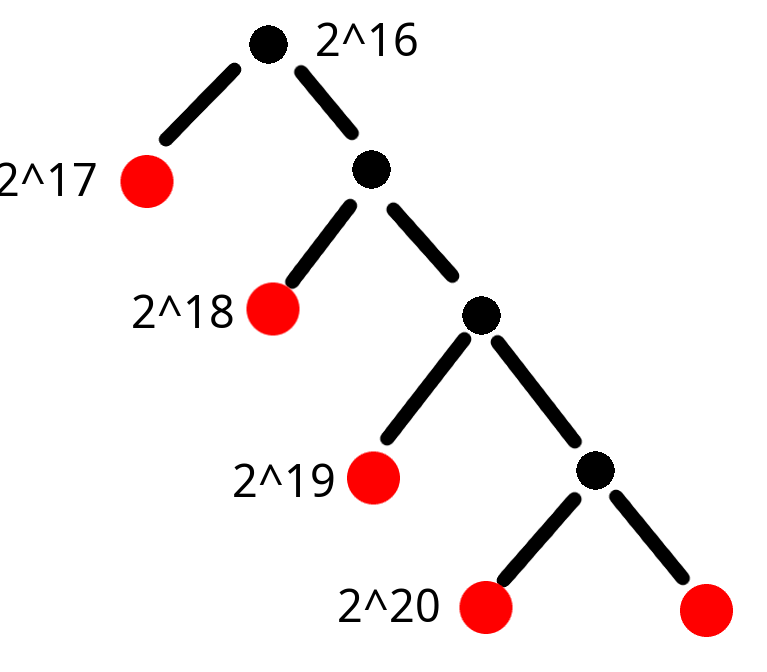
\includegraphics[scale=0.4]{./L01Z02.png}
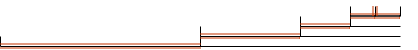
\includegraphics[scale=0.4]{./L01Z02czII.png}
\end{center}
imo wygodniejszy sposób reprezentacji tego zadania to "kubełki" (ten po prawej).
\item{Tablica routingu zawiera następujące wpisy (podsieć → dokąd wysłać):
\begin{itemize}[label=$\blacktriangleright$]
	\item 0.0.0.0/0 → do routera A
	\item 10.0.0.0/23 → do routera B
	\item 10.0.2.0/24 → do routera B
	\item 10.0.3.0/24 → do routera B
	\item 10.0.1.0/24 → do routera C
	\item 10.0.0.128/25 → do routera B
	\item 10.0.1.8/29 → do routera B
	\item 10.0.1.16/29 → do routera B
	\item 10.0.1.24/29 → do routera B
\end{itemize}
Napisz równoważną tablicę routingu zawierającą jak najmniej wpisów}\\\\
to co będziemy chcieli zrobić, to "zlepić" odpowiednie adresy, o ile są one sąsiadujące, oraz wykluczyć "nadmiarowe" adresy.
Możemy zauważyć że:\\
 \null \quad koniec podsieci trzeciej (10.0.2.255) znajduje się obok sieci czwartej (10.0.3.0), tak więc możemy scalić (rozmiar maski maleje nam o 1);\\
  \null \quad koniec podsieci drugiej (10.0.1.255) znajduje się obok sieci trzeciej (10.0.2.0), tak więc możemy je złączyć (rozmiar maski maleje nam o 1);\\
 \null \quad podsieć szósta w całości znajduje się w podsieci drugiej, tak więc możemy pominąć;\\
 \null \quad podsieć ósma i dziewiąta (odpowiednio 10.0.1.23 i 10.0.1.24) można połączyć ze sobą;\\
 \null \quad podsieci siódmej nie możemy podłączyć, ponieważ nie potrafimy utworzyć takiej jednoznacznej maski.\\
  Ostatecznie po wszystkich edycjach uzyskamy:
 \begin{itemize}[label=$\blacktriangleright$]
	\item 0.0.0.0/0 → do routera A
	\item 10.0.0.0/22 → do routera B
	\item 10.0.1.0/24 → do routera C
	\item 10.0.1.8/29 → do routera B
	\item 10.0.1.16/28 → do routera B
\end{itemize}
 \item{Wykonaj powyższe zadanie dla tablicy
 \begin{itemize}[label=$\blacktriangleright$]
	\item 0.0.0.0/0 → do routera A
	\item 10.0.0.0/8 → do routera B
	\item 10.3.0.0/24 → do routera C
	\item 10.3.0.32/27 → do routera B
	\item 10.3.0.64/27 → do routera B
	\item 10.3.0.96/27 → do routera B
\end{itemize}}
\null \quad Dwa ostatnie adresy możemy scalić, uzyskując 10.3.0.64/26\\
\null \quad Mimo że może się zdawać, że nie potafimy już bardziej tego złączyć, możemy zauważyć jedną rzecz. rozbijając router C na dwa osobne wpisy w tablicy routingu, będziemy mogli pozbyć aż trzy (!) ostatnie wpisy (lub dwa, jeżeli już się scaliło). Niezależnie od tego czy scalaliśmy wcześniej, efekt jest zadowalający.
\null \quad	tak więc adres C zakrywa odpowiednio od 10.3.0.0 do 10.3.0.31 i od 10.3.0.128 do 10.3.0.255.
\null \quad Tak więc nasza odpowiedź to:
\begin{itemize}[label=$\blacktriangleright$]
	\item 0.0.0.0/0 → do routera A
	\item 10.0.0.0/8 → do routera B
	\item 10.3.0.0/27 → do routera C
	\item 10.3.0.128/25 → do routera C
\end{itemize}
\item{Jak uporządkować wpisy w tablicy routingu, żeby zasada najlepszego dopasowania odpowiadała wyborowi „pierwszy pasujący” (tj. przeglądaniu tablicy od początku do końca aż do momentu napotkania dowolnej pasującej reguły)? Odpowiedź uzasadnij formalnie.}\\
wiemy że tablice routingu kierują się regułą najdłuższego prefiksu dla wielu identycznych reguł. Tak więc nasze uporządkowanie listy powinny być w kolejności malejącej względem długości prefiksa.\\
\textbf{Dowód:} Załóżmy nie wprost, że zachłanny wynik z posortowanej tablicy daje nam wpis gorszy od najlepszego możliwego. rozpatrzmy trzy przypadki:
\begin{itemize}
	\item prefiks najlepszej odpowiedzi jest dłuższy od zachłannej odpowiedzi.\\
	\null \quad to stwierdzenie nie może być prawdziwe, ponieważ zachłannie bierzemy prawidłowy wpis z najdłuższym możliwym prefiksem;
	\item prefiks najlepszej odpowiedzi jest równy wynikowi zachłannemu.\\
	\null \quad w takim przypadku odpowiedź najlepsza jest ta sama, co zachłanny wynik, ponieważ wpisy dla masek tej samej długości nie nachodzą na siebie (n pierwszych bitów jest "nieedytowalna");
	\item prefiks najlepszej odpowiedzi jest krótszy od wyniku zachłannego.\\
	\null \quad Nie jest to możliwe, ponieważ zgodnie z regułą wybieramy adres pasujący z najdłuższym możliwym prefiksem.
\end{itemize}
Dochodzimy do sprzeczności. Tak więc najlepszy wynik to zachłanny, co kończy nam dowód.
\item {W podanej niżej sieci tablice routingu budowane są za pomocą algorytmu wektora odległości. Pokaż (krok po kroku), jak będzie się to odbywać. W ilu krokach zostanie osiągnięty stan stabilny?}\\
\begin{center}
	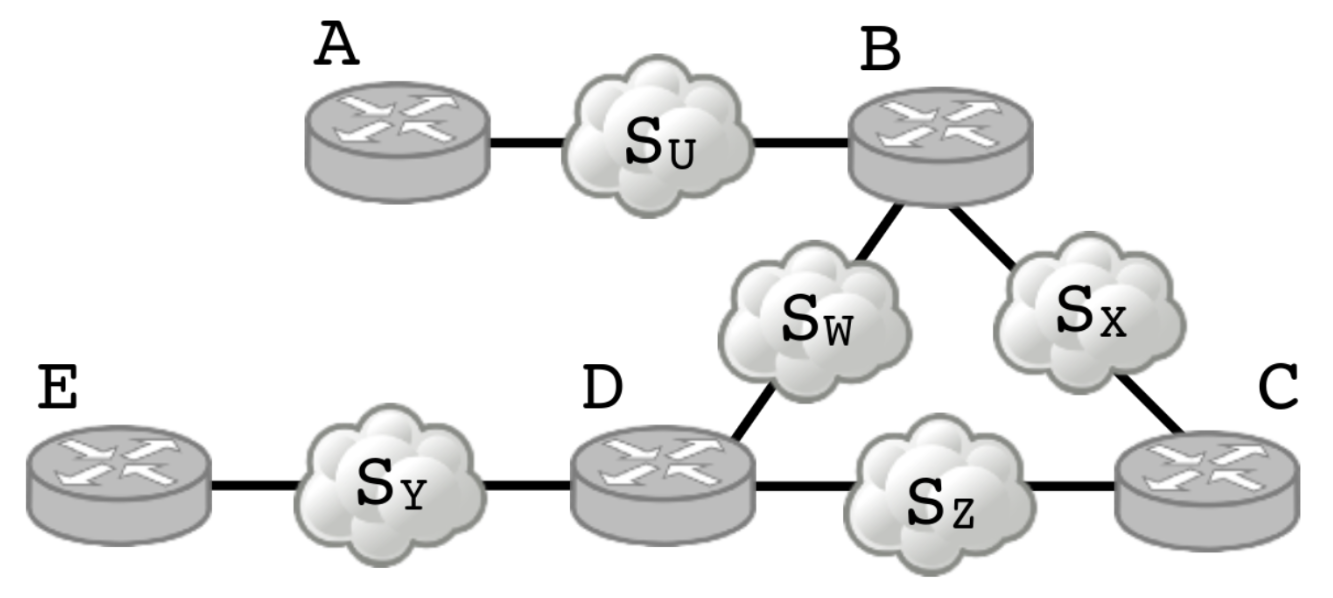
\includegraphics[scale=0.2]{./L01Z06.png}
\end{center}
Algorytm wektora odległości polega na okresowym powiadamianiu sąsiednich routerów o całej swojej tablicy przekazywania i aktualizowaniu na tej bazie.\\
Na początku uzupełnijmy wszystkich sąsiadów
\begin{center}
	\begin{tabular}{c||c|c|c|c|c|} 
	  &$A$&$B$&$C$&$D$&$E$\\
	 \hline \hline
	 do $S_u$&1&1& & & \\ 
	 \hline
	 do $S_w$& &1& &1& \\ 
	 \hline
	 do $S_x$& &1&1& & \\ 
	 \hline
	 do $S_z$& & &1&1& \\ 
	 \hline
	 do $S_y$& & & &1&1\\ 
	 \hline \hline
	\end{tabular}
	\begin{tabular}{c||c|c|c|c|c|} 
	  &$A$&$B$&$C$&$D$&$E$\\
	 \hline \hline
	 do $S_u$&1&1&2(via B)&2(via B)& \\ 
	 \hline
	 do $S_w$&2(via B)&1&2(via B)&1&2(via D)\\ 
	 \hline
	 do $S_x$&2(via B)&1&1&2(via C)& \\ 
	 \hline
	 do $S_z$& &2(via C)&1&1&2(via D)\\ 
	 \hline
	 do $S_y$& &2(via D)&2(via D)&1&1\\ 
	 \hline \hline
	\end{tabular}\\
	\vspace{1em}
	\begin{tabular}{c||c|c|c|c|c|} 
	  &$A$&$B$&$C$&$D$&$E$\\
	 \hline \hline
	 do $S_u$&1&1&2(via B)&2(via B)&3(via D)\\ 
	 \hline
	 do $S_w$&2(via B)&1&2(via B)&1&2(via D)\\ 
	 \hline
	 do $S_x$&2(via B)&1&1&2(via C)&3(via D)\\ 
	 \hline
	 do $S_z$&3(via B)&2(via C)&1&1&2(via D)\\ 
	 \hline
	 do $S_y$&3(via B) &2(via D)&2(via D)&1&1\\ 
	 \hline \hline
	\end{tabular}
\end{center}
\item{Załóżmy, że w powyższej sieci tablice routingu zostały już zbudowane. Co będzie się działo (krok po kroku), jeśli zostanie dodana sieć $S_Q$ łącząca routery A i E ?}
po dodaniu w pierwszym kroku router A i E uzyskają informację że potrafią dotrzeć do $S_Q$ ścieżką długości jeden. W drugim kroku tablica uzupełni się dla reszty routerów względem routera A lub E.
\begin{center}
\begin{tabular}{c||c|c|c|c|c|} 
	  &$A$&$B$&$C$&$D$&$E$\\
	 \hline \hline
	 do $S_u$&1&1&2(via B)&2(via B)&3(via D)\\ 
	 \hline
	 do $S_w$&2(via B)&1&2(via B)&1&2(via D)\\ 
	 \hline
	 do $S_x$&2(via B)&1&1&2(via C)&3(via D)\\ 
	 \hline
	 do $S_z$&3(via B)&2(via C)&1&1&2(via D)\\ 
	 \hline
	 do $S_y$&3(via B) &2(via D)&2(via D)&1&1\\ 
	 \hline 
	 do $S_q$&1& & & &1\\
	 \hline \hline
	 
\end{tabular}\\
	 \vspace{1em}
\begin{tabular}{c||c|c|c|c|c|} 
	  &$A$&$B$&$C$&$D$&$E$\\
	 \hline \hline
	 do $S_u$&1&1&2(via B)&2(via B)&3(via D)\\ 
	 \hline
	 do $S_w$&2(via B)&1&2(via B)&1&2(via D)\\ 
	 \hline
	 do $S_x$&2(via B)&1&1&2(via C)&3(via D)\\ 
	 \hline
	 do $S_z$&3(via B)&2(via C)&1&1&2(via D)\\ 
	 \hline
	 do $S_y$&3(via B) &2(via D)&2(via D)&1&1\\ 
	 \hline 
	 do $S_q$&1&2(via A)&3(via A)&2(via E)&1\\
	 \hline \hline
\end{tabular}
\end{center}

\item{W przedstawionej poniżej sieci uszkodzeniu ulega połączenie między routerami D i E . Załóżmy, że w sieci działa algorytm wektora odległości wykorzystujący technikę zatruwania ścieżki zwrotnej (poison reverse). Pokaż — opisując krok po kroku jakie komunikaty są przesyłane między routerami
— że może powstać cykl w routingu.}
\begin{center}
	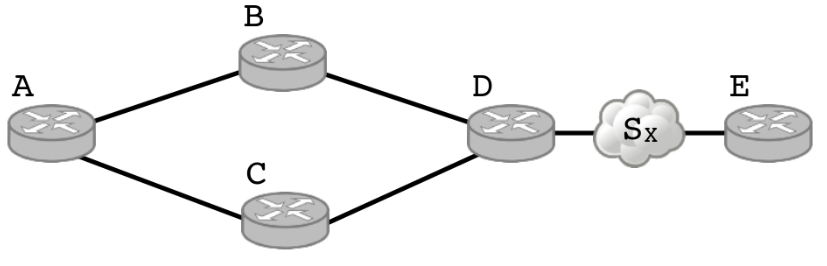
\includegraphics[scale=0.2]{./L01Z08.png}
\end{center}
poison reverse polega na wykorzystywaniu informacji skąd przybyliśmy aby zabezpieczyć się przed wieczną pętlą. Na początku tablica wygląda następująco:
\begin{center}
\begin{tabular}{c||c|c|c|c|c|} 
	  &$A$&$B$&$C$&$D$&$E$\\
	 \hline \hline
	 do $S_x$&3(via B)&2(viad D)&2(via D)&1&1\\ 
	 \hline \hline
\end{tabular}
\end{center} $S_x$ podana sieć będzie początkowo wyglądać:
\begin{center}
\begin{tabular}{c||c|c|c|c|c|} 
	  &$A$&$B$&$C$&$D$&$E$\\
	 \hline \hline
	 do $S_x$&3(via B)&2(viad D)&2(via D)&&\\ 
	 \hline \hline
\end{tabular}
\end{center} 
w kolejnym kroku B ustawi wartość dla D równą nieskończoność
\begin{center}
\begin{tabular}{c||c|c|c|c|c|} 
	  &$A$&$B$&$C$&$D$&$E$\\
	 \hline \hline
	 do $S_x$&3(via B)&2(viad D)&2(via D)&$\inf$&\\ 
	 \hline \hline
\end{tabular}
\end{center}
następnie B i C zostaną ustawione na nieskończoność
\begin{center}
\begin{tabular}{c||c|c|c|c|c|} 
	  &$A$&$B$&$C$&$D$&$E$\\
	 \hline \hline
	 do $S_x$&3(via B)&$\inf$&$\inf$&$\inf$&\\ 
	 \hline \hline
\end{tabular}
\end{center} 
aby na końcu ustawić w A nieskończoność
\begin{center}
\begin{tabular}{c||c|c|c|c|c|} 
	  &$A$&$B$&$C$&$D$&$E$\\
	 \hline \hline
	 do $S_x$&$\inf$&$\inf$&$\inf$&$\inf$&\\ 
	 \hline \hline
\end{tabular}
\end{center} 
\item{Pokaż, że przy wykorzystaniu algorytmu stanu łączy też może powstać cykl w routingu. W tym celu skonstruuj sieć z dwoma wyróżnionymi, sąsiadującymi ze sobą routerami A i B. Załóż, że wszystkie routery znają graf całej sieci. W pewnym momencie łącze między A i B ulega awarii, o czym A i B od razu się dowiadują. Zalewają one sieć odpowiednią aktualizacją. Pokaż, że w okresie propagowania tej aktualizacji (kiedy dotarła ona już do części routerów a do części nie) może powstać cykl w routingu}\\

\end{enumerate}

 \end{document}
